% This is text associated with the open textbook "Open Electromagnetics"
% See immediately below for author, date
% This work is licensed under the Creative Commons Attribution-ShareAlike 4.0 International License. (CC BY-SA 4.0) 
% To view a copy of the license, visit http://creativecommons.org/licenses/by-sa/4.0/

%ORB TITLE Telegrapher's Equations
%ORB AUTHOR 0        # S.W. Ellingson, Virginia Tech (ellingson@vt.edu)
%ORB DATE 20180802   # yyyymmdd
%ORB ABSTRACT Development of the telegrapher's equations given the lumped-element model.

\label{m0079_Telegraphers_Equations} % <-- Must match name of this file and module directory name.  Don't mess with this!
\index{telegrapher's equations|(}

In this section, we derive the equations that govern the potential $v(z,t)$ and current $i(z,t)$ along a transmission line that is oriented along the $z$ axis.  
For this, we will employ the lumped-element model developed in Section~\ref{m0029_Lumped-Element_Model}.

To begin, we define voltages and currents as shown in Figure~\ref{m0079_fLumpedElementModel}.  
%
\begin{figure}[b!]
\begin{center}
\pdftooltip{{  % note double brace
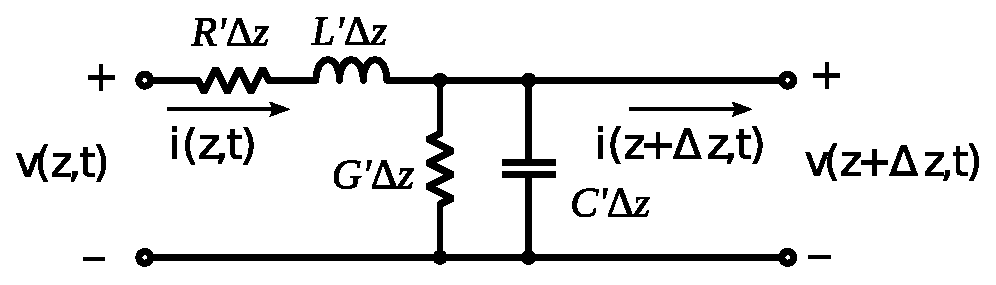
\includegraphics[width=\columnwidth]{modules/m0079_Transmission_line_element_se170804.eps}
% https://commons.wikimedia.org/wiki/File:Transmission_line_element.svg (modified)
}}{A lumped-element equivalent circuit model the same as an earlier figure. On the left side open node, the potential v(z,t) is shown with positive terminal applied to the resistor.  Underneath the series resistor, a right pointing arrow is labeled i(z,t). On the right side of the circuit, the voltage potential is given as v( z + Delta z, t ). On the positive exit node, an arrow labeled i( z + Delta z, t ) points to the right.}
\end{center} 
\centerline{\scriptsize 
\copyright~\hyperref[m0079_fLumpedElementModel_Credit]{Omegatron} 
\href{https://creativecommons.org/licenses/by-sa/3.0/deed.en}{CC BY~SA 3.0 Unported} (modified) 
} 
\caption{
\label{m0079_fLumpedElementModel}
Lumped-element equivalent circuit transmission line model, annotated with sign conventions for potentials and currents.
}
\end{figure}
%
We assign the variables $v(z,t)$ and $i(z,t)$ to represent the potential and current on the left side of the segment, with reference polarity and direction as shown in the figure.
Similarly we assign the variables $v(z+\Delta z,t)$ and $i(z+\Delta z,t)$ to represent the potential and current on the right side of the segment, again with reference polarity and direction as shown in the figure.
Applying Kirchoff's voltage law from the left port, through $R'\Delta z$ and $L'\Delta z$, and returning via the right port, we obtain:
%
\begin{multline}
v(z,t) - \left( R'\Delta z \right) i(z,t) - \left( L' \Delta z\right) \frac{\partial}{\partial t} i(z,t) \\ - v(z+\Delta z,t) = 0
\end{multline}
%
Moving terms referring to current to the right side of the equation and then dividing through by $\Delta z$, we obtain
%
\begin{multline}
-\frac{v(z+\Delta z,t)-v(z,t)}{\Delta z} = \\
R'~i(z,t) + L'~\frac{\partial}{\partial t} i(z,t)
\end{multline}
%
Then taking the limit as $\Delta z \rightarrow 0$:
%
\begin{multline}
\boxed{
-\frac{\partial}{\partial z} v(z,t) = 
R'~i(z,t) + L'~\frac{\partial}{\partial t} i(z,t)
}
\label{m0079_eTelegraphersEquation1}
\end{multline}

Applying Kirchoff's current law at the right port, we obtain:
%
\begin{multline}
i(z,t) - \left( G'\Delta z \right) v(z+\Delta z,t) - \left( C' \Delta z\right) \frac{\partial}{\partial t} v(z+\Delta z,t) \\ - i(z+\Delta z,t) = 0
\end{multline}
%
Moving terms referring to potential to the right side of the equation and then dividing through by $\Delta z$, we obtain
%
\begin{multline}
-\frac{i(z+\Delta z,t)-i(z,t)}{\Delta z} = \\
G'~v(z+\Delta z,t) + C'~\frac{\partial}{\partial t} v(z+\Delta z,t)
\end{multline}
%
Taking the limit as $\Delta z \rightarrow 0$:
%
\begin{multline}
\boxed{
-\frac{\partial}{\partial z} i(z,t) = 
G'~v(z,t) + C'~\frac{\partial}{\partial t} v(z,t)
}
\label{m0079_eTelegraphersEquation2}
\end{multline}
%
%ORB HIGHLIGHT
\begin{mdframed}[backgroundcolor=yellow!20,nobreak=true] 
Equations~\ref{m0079_eTelegraphersEquation1} and \ref{m0079_eTelegraphersEquation2} are the \emph{telegrapher's equations}.  These coupled (simultaneous) differential equations can be solved for $v(z,t)$ and $i(z,t)$ given $R'$, $G'$, $L'$, $C'$ and suitable boundary conditions.
\end{mdframed}

The time-domain telegrapher's equations are usually more than we need or want.  If we are only interested in the response to a sinusoidal stimulus, then considerable simplification is possible using phasor representation.\footnote{For a refresher on phasor analysis, see Section~\ref{m0033_Phasors}.}  First we define phasors $\widetilde{V}(z)$ and $\widetilde{I}(z)$ through the usual relationship:
%
\begin{equation}
v(z,t) = \mbox{Re}\left\{\widetilde{V}(z) ~ e^{j\omega t} \right\}
\end{equation}
%
\begin{equation}
i(z,t) = \mbox{Re}\left\{\widetilde{I}(z) ~ e^{j\omega t} \right\}
\end{equation}  
%
Now we see:
%
\begin{equation}
\begin{split}
\frac{\partial}{\partial z} v(z,t) & = \frac{\partial}{\partial z} \mbox{Re}\left\{\widetilde{V}(z) ~ e^{j\omega t} \right\} \nonumber \\
                                   & = \mbox{Re}\left\{ \left[ \frac{\partial}{\partial z} \widetilde{V}(z) \right] ~ e^{j\omega t} \right\}
\end{split}
\end{equation}
%
In other words, $\partial v(z,t)/\partial z$ expressed in phasor representation is simply $\partial \widetilde{V}(z)/\partial z$; and 
%
\begin{equation}
\begin{split}
\frac{\partial}{\partial t} i(z,t) & = \frac{\partial}{\partial t} \mbox{Re}\left\{\widetilde{I}(z) ~ e^{j\omega t} \right\} \nonumber \\
                                   & = \mbox{Re}\left\{ \frac{\partial}{\partial t} \left[ \widetilde{I}(z) e^{j\omega t} \right] \right\} \nonumber \\
                                   & = \mbox{Re}\left\{ \left[ j\omega \widetilde{I}(z) \right] e^{j\omega t} \right\}
\end{split}
\end{equation}
%
In other words, $\partial i(z,t)/\partial t$ expressed in phasor representation is $j\omega \widetilde{I}(z)$.
Therefore, Equation~\ref{m0079_eTelegraphersEquation1} expressed in phasor representation is:
%
\begin{equation}
\boxed{
-\frac{\partial}{\partial z} \widetilde{V}(z) = \left[ R' + j\omega L' \right]~\widetilde{I}(z)
}
\label{m0079_eTelegraphersEquation1p}
\end{equation}
%
Following the same procedure, Equation~\ref{m0079_eTelegraphersEquation2} expressed in phasor representation is found to be:
%
\begin{equation}
\boxed{
-\frac{\partial}{\partial z} \widetilde{I}(z) = \left[ G' + j\omega C' \right]~\widetilde{V}(z)
}
\label{m0079_eTelegraphersEquation2p}
\end{equation}
%
%ORB HIGHLIGHT
\begin{mdframed}[backgroundcolor=yellow!20,nobreak=true] 
Equations~\ref{m0079_eTelegraphersEquation1p} and \ref{m0079_eTelegraphersEquation2p} are the telegrapher's equations in phasor representation. 
\end{mdframed}
%
The principal advantage of these equations over the time-domain versions is that we no longer need to contend with derivatives with respect to time -- only derivatives with respect to distance remain.
This considerably simplifies the equations.

%%%%%%%%%%%%%%%%%%%%%%%%%%%%%%%%%%%%%%%%%%%

{\bf Additional Reading:}
\begin{itemize}
\item ``\href{https://en.wikipedia.org/wiki/Telegrapher's_equations}{Telegrapher's equations}'' on Wikipedia.
\item ``\href{https://en.wikipedia.org/wiki/Kirchhoff's_circuit_laws}{Kirchhoff's circuit laws}'' on Wikipedia.
\end{itemize}

\index{telegrapher's equations|)}




